\section{Model analysis}

\begin{definition}[\textit{Computationally Stronger}]
    A model $A$ is said to be computationally stronger than model $B$ ($A \geq B$) if any algorithm written for $B$ can run unchanged on $A$ with the same parallel time and basic properties.
\end{definition}
\begin{lemma}
    Assume $P^\prime<P$, and same size of shared memory.
    Any problem that can be solved for a $P$-processor PRAM in $T$ steps can be solved in a $P^\prime$ processor PRAM in $T^\prime=O(T\frac{P}{P^\prime})$ steps
\end{lemma}
\begin{lemma}
    Assume $M^\prime < M$. 
    Any problem that can be solved for a $P$-processor and $M$-cell PRAM in $T$ steps can be solved on a $\max(P, M^\prime)$-processor $M^\prime$-cell PRAM in $\mathcal{O}\left(T\frac{M}{M^\prime}\right)$ steps.
\end{lemma}

The direct implementation of a PRAM on real hardware poses certain challenges due to its theoretical nature. 
Despite this, PRAM algorithms can be adapted for practical systems, allowing the abstract model to influence real-world designs.

\subsection{Amdahl law}
In parallel computing, we consider two types of program segments: serial segments and parallelizable segments. 
The total execution time depends on the proportion of each.
\begin{figure}[H]
    \centering
    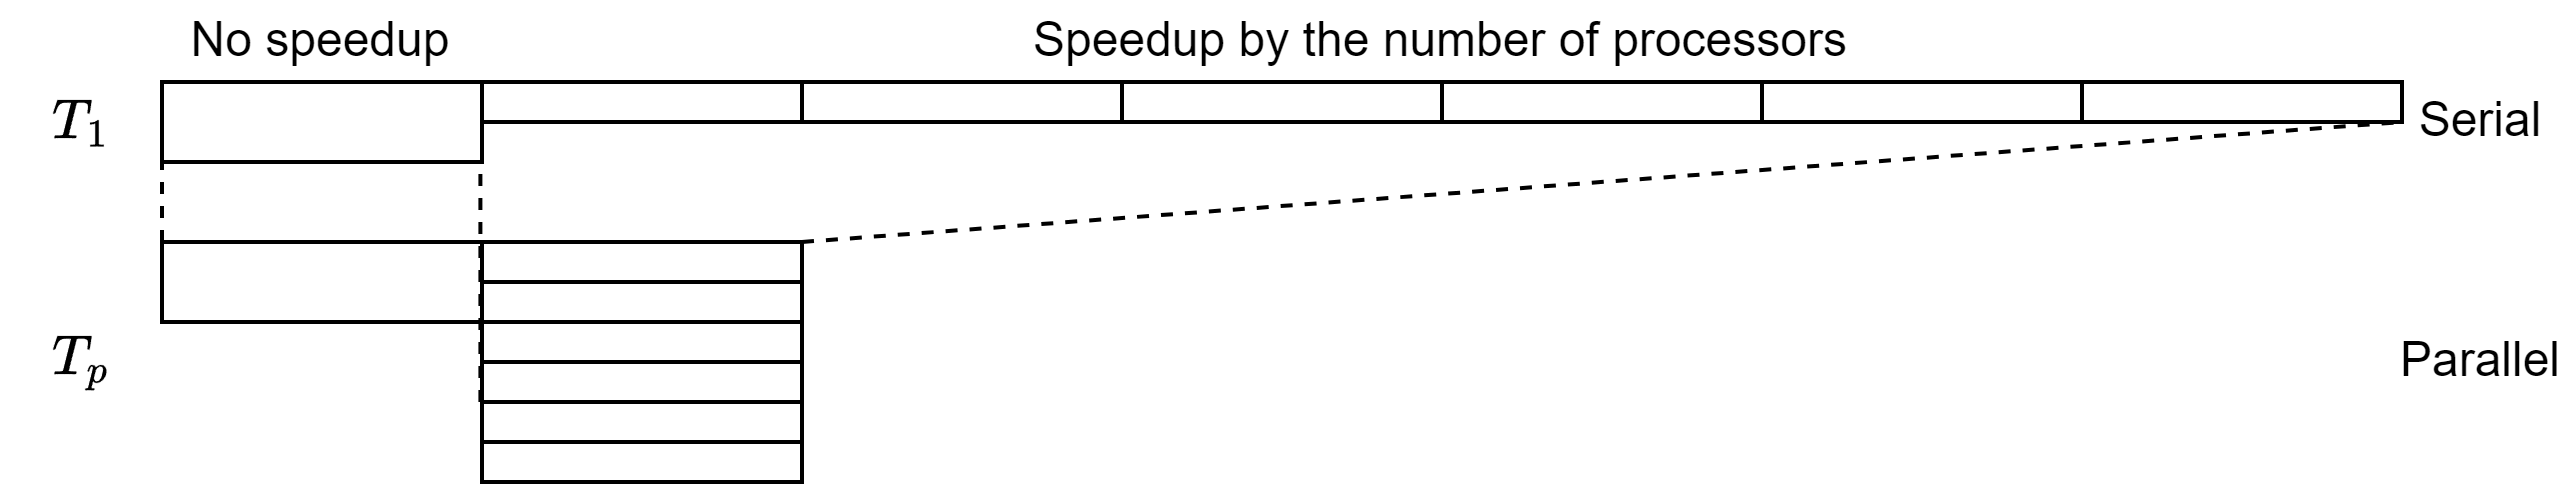
\includegraphics[width=0.8\linewidth]{images/am.png}
    \caption{Serial and parallel models}
\end{figure}
When using more than one processor, the speedup is always less than the number of processors. 
In a program, the parallelizable portion is often represented by a fixed fraction $f$. 
\begin{figure}[H]
    \centering
    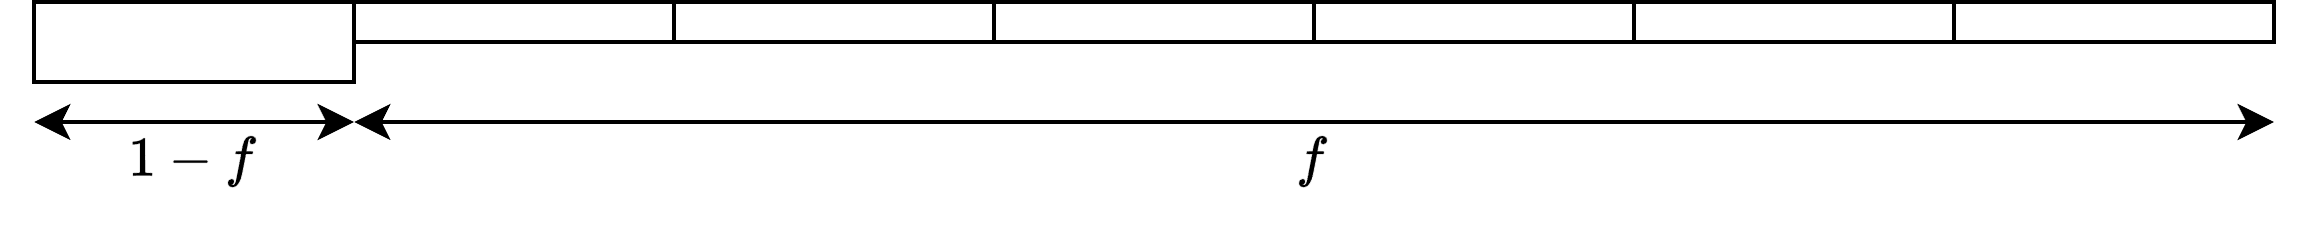
\includegraphics[width=0.8\linewidth]{images/am1.png}
    \caption{Serial model}
\end{figure}
Using the serial version of the model, the speedup function $\text{SU}(p,f)$ is derived as follows:
\[\text{SU}(p,f)=\dfrac{1}{(1-f)+\frac{f}{p}}\]
As the number of processors $p$ approaches infinity, the speedup is limited by the serial portion:
\[\lim_{p\rightarrow\infty}\text{SU}(p,f)=\dfrac{1}{1-f}\]
This shows that even with an infinite number of processors, the maximum speedup is constrained by the serial fraction of the program. 

\subsection{Gustafson law}
In contrast to Amdahl's Law, John Gustafson proposed a different view in 1988, challenging the assumption that the parallelizable portion of a program remains fixed. 
Key differences include:
\begin{itemize}
    \item The parallelizable portion of the program is not a fixed fraction.
    \item Absolute serial time is fixed, while the problem size grows to exploit more processors.
\end{itemize}
Amdahl's law is based on a fixed-size model, while Gustafson's law operates on a fixed-time model, where the problem grows with increased processing power.
The speedup in Gustafson's model is expressed as:
\[\text{SU}(p)=s+p(1-s)\]
Here, $s$ is the fixed serial portion of the program.
As a result, this model suggests linear speedup is possible as the number of processors increases, especially for highly parallelizable tasks. 
Gustafson's law is empirically applicable to large-scale parallel algorithms, where increasing computational power enables solving larger and more complex problems within the same time frame.